\documentclass[12pt]{article}
\usepackage{graphicx}
\usepackage[none]{hyphenat}
\usepackage{graphicx}
\usepackage{listings}
\usepackage[english]{babel}
\usepackage{graphicx}
\usepackage{caption} 
\usepackage{booktabs}
\usepackage{array}
\usepackage{amssymb} % for \because
\usepackage{amsmath}   % for having text in math mode
\usepackage{extarrows} % for Row operations arrows
\usepackage{listings}
\lstset{
  frame=single,
  breaklines=true
}
\usepackage{hyperref}
\usepackage{bm}
  
%Following 2 lines were added to remove the blank page at the beginning
\usepackage{atbegshi}% http://ctan.org/pkg/atbegshi
\AtBeginDocument{\AtBeginShipoutNext{\AtBeginShipoutDiscard}}
\usepackage{gensymb}


%New macro definitions
\newcommand{\mydet}[1]{\ensuremath{\begin{vmatrix}#1\end{vmatrix}}}
\providecommand{\brak}[1]{\ensuremath{\left(#1\right)}}
\providecommand{\sbrak}[1]{\ensuremath{{}\left[#1\right]}}
\providecommand{\norm}[1]{\left\lVert#1\right\rVert}
\providecommand{\abs}[1]{\left\vert#1\right\vert}
\newcommand{\solution}{\noindent \textbf{Solution: }}
\newcommand{\myvec}[1]{\ensuremath{\begin{pmatrix}#1\end{pmatrix}}}
\let\vec\mathbf


\begin{document}

\begin{center}
\title{\textbf{3D Lines}}
\date{\vspace{-5ex}} %Not to print date automatically
\maketitle
\end{center}
\setcounter{page}{1}

\section{JEE Maths - 65 C-1}
This is Problem-30 
\begin{enumerate}
\item Find the shortest distance between the lines $\frac{x-1}{2} = \frac{y+1}{3}=z$ and $\frac{x+1}{5} = \frac{y-2}{1}; z=2 $ 

\solution 
The given equation can be written as
\begin{align}
	\label{eq:Eq1}
	\frac{x-1}{2} &= \frac{y+1}{3}=\frac{z-0}{1}\\ 
	\label{eq:Eq2}
	\frac{x+1}{5} &= \frac{y-2}{1}= \frac{z-2}{0} \\ 
	\implies 
	\vec{x} &= \myvec{1\\-1\\0} + \lambda_1\myvec{2\\3\\1}\\
        \vec{x} &= \myvec{-1\\2\\2} + \lambda_2\myvec{5\\1\\0} \\
	\vec{x_1} &= \myvec{1\\-1\\0},  
	\vec{x_2} = \myvec{-1\\2\\2},  
	\vec{m_1} = \myvec{2\\3\\1},
	\vec{m_2} = \myvec{5\\1\\0} 
\end{align}
We first check whether the given lines are skew. The lines 
\begin{align}
	\label{eq:Eq3}
	\vec{x} = \vec{x_1} + \lambda_1\vec{m_1},\, \vec{x} = \vec{x_2} + \lambda_2\vec{m_2} 
\end{align}
intersect if
\begin{align}
	\vec{M}{\lambda} &= \vec{x_2} - \vec{x_1}\\
	\vec{M} &\triangleq \myvec{\vec{m_1} & \vec{m_2}} \\
	\bm{\lambda} &\triangleq \myvec{\lambda_1\\-\lambda_2}
\end{align}
Here we have,
\begin{align}
	\vec{M} = \myvec{2&5\\3&1\\1&0},
	\vec{x_2} - \vec{x_1} = \myvec{-2\\3\\2}  \\
	\label{eq:Eq4}
        \implies \myvec{2&5\\3&1\\1&0}\bm{\lambda} = \myvec{-2\\3\\2}
\end{align}
Let us check whether the equation \eqref{eq:Eq4} has a solution.

The augmented matrix is given by,
\begin{align}
	\myvec{2&5&\vrule&-2\\3&1&\vrule&3\\1&0&\vrule&2}
	\xleftrightarrow[R_3 \leftarrow R_3 - \frac{1}{2}R_1]{R_2 \leftarrow R_2 - \frac{3}{2}R_1}\\
	\myvec{2&5&\vrule&-2\\&&\vrule\\0&-\frac{13}{2}&\vrule&6\\&&\vrule\\0&-\frac{5}{2}&\vrule&3}
	\xleftrightarrow{R_3 \leftarrow R_3 - \frac{5}{13}R_2}\\
	\myvec{2&5&\vrule&-2\\&&\vrule\\0&-\frac{13}{2}&\vrule&6\\&&\vrule\\0&0&\vrule&\frac{9}{13}}
\end{align}
The rank of the matrix is 3. So the given lines are skew.
The closest points on two skew lines defined by \eqref{eq:Eq3} are given by 
\begin{align}
	\vec{M}^\top \vec{M}\bm{\lambda} &= \vec{M}^\top\brak{\vec{x_2}-\vec{x_1}}\\
	\implies \myvec{2&3&1\\5&1&0}\myvec{2&5\\3&1\\1&0}\bm\lambda &= \myvec{2&3&1\\5&1&0} \myvec{-2\\3\\2} \\
	\label{eq:Eq5}
	\implies \myvec{14&13\\13&26}\bm{\lambda} &= \myvec{7\\-7}
\end{align}
The augmented matrix of the above equation \eqref{eq:Eq5} given by,
\begin{align}
	\myvec{14&13&\vrule&7\\13&26&\vrule&-7}
	\xleftrightarrow{R_2 \leftarrow R_2 - \frac{13}{14}R_1} \\
	\myvec{14&13&\vrule&7 \\&& \vrule\\ 0&\frac{195}{14}&\vrule&\frac{-27}{2}}
	\xleftrightarrow{R_1 \leftarrow \brak{R_1}-\frac{14}{15}R_2} \\
	\myvec{14&0&\vrule&\frac{98}{5}\\&&\vrule\\0&\frac{195}{14}&\vrule&\frac{-27}{2}} 
	\xleftrightarrow[R_2 \leftarrow \frac{14}{195}R_2]{R_1 \leftarrow \frac{1}{14} \brak{R_1}}\\
	\myvec{1&0&\vrule&\frac{7}{5}\\&&\vrule\\0&1&\vrule&\frac{-63}{65}}
\end{align}
resulting
\begin{align}
 	\myvec{\lambda_1\\-\lambda_2} &= \myvec{\frac{7}{5}\\\\\frac{-63}{65}}
\end{align}
The closest points $\vec{A}$ on line $l_1$ and $\vec{B}$ on line $l_2$ are given by,
\begin{align}
	\vec{A} &= \vec{x_1} + \lambda_1\vec{m_1}
	= \myvec{1\\-1\\0} + \frac{7}{5}\myvec{2\\3\\1} = \myvec{\frac{19}{5}\\ \\ \frac{16}{5}\\ \\ \frac{7}{5}}\\
	\vec{B} &= \vec{x_2} + \lambda_2\vec{m_2}
	= \myvec{-1\\2\\2} + \frac{63}{65}\myvec{5\\1\\0} = \myvec{\frac{50}{13}\\ \\ \frac{193}{65}\\ \\ 2} 
\end{align}
The minimum distance between the lines is given by
\begin{align}
	\norm{\vec{B}-\vec{A}} &= \norm{\myvec{\frac{3}{65}\\\\\frac{-15}{65}\\\\\frac{3}{5}}}
	= 3\sqrt{\frac{3}{65}} = 0.6445 \text{ units}
\end{align}
The relevant figure is shown in \ref{fig:Fig1}. 
\begin{figure}[!h]
	\begin{center}
		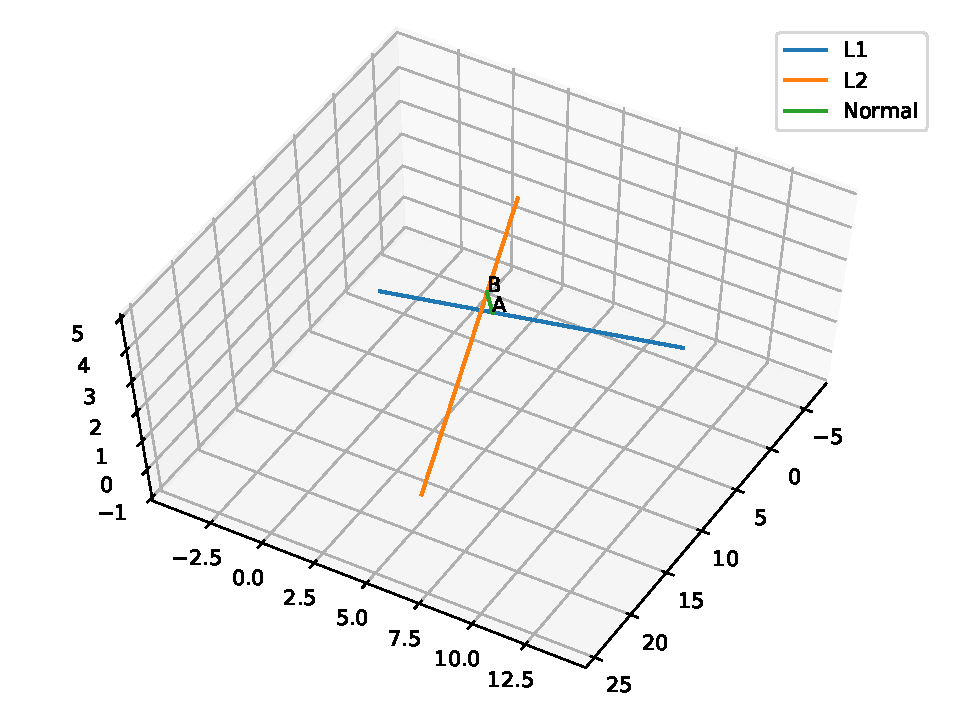
\includegraphics[width=\columnwidth]{figs/problem30.pdf}
	\end{center}
\caption{}
\label{fig:Fig1}
\end{figure}
\end{enumerate}
\end{document}
